% SASYR 2025 - Template based on:
% samplepaper.tex, a sample chapter demonstrating the
% LLNCS macro package for Springer Computer Science proceedings;
% Version 2.20 of 2017/10/04
%
\documentclass[runningheads]{llncs}
%
\usepackage{graphicx}
\usepackage{ctex}
\usepackage{lipsum}
\usepackage{amsmath}
\usepackage{tikz}
\usepackage{url}
\usetikzlibrary{positioning}
\usetikzlibrary{shapes.geometric}
\usetikzlibrary{shapes.arrows}
\usetikzlibrary{arrows.meta}
% Used for displaying a sample figure. If possible, figure files should
% be included in EPS format.
%
% If you use the hyperref package, please uncomment the following line
% to display URLs in blue roman font according to Springer's eBook style:
% \renewcommand\UrlFont{\color{blue}\rmfamily}

\begin{document}
%
\title{围串标聚类 Phase 0.1}
%
%\titlerunning{Abbreviated paper title}
% If the paper title is too long for the running head, you can set
% an abbreviated paper title here
%
\author{Pengfei}
%
% \authorrunning{F. Author et al.}
% First names are abbreviated in the running head.
% If there are more than two authors, 'et al.' is used.
%
\institute{
% \email{author@ipvc.pt}\\
% \and
% CeDRI, Instituto Politécnico de Bragança, Portugal\\
% \email{author@ipb.pt}
% \and
% 2AI, Instituto Politécnico do Cávado e do Ave, IPCA, Portugal\\
% \email{author@ipca.pt}
% \and
% GECAD, Instituto Politécnico do Porto, IPP, Portugal\\
\email{pengfeigaothu@gmail.com}
}
%
\maketitle              % typeset the header of the contribution
%
\begin{abstract}
聚类算法方案 \\


\keywords{Clustering}
\end{abstract}
%
%
%
\section{整体目标}
根据历史投标数据,对公司进行聚类,将有可能涉及围串标的公司聚成一个类。

对聚类算法的要求:
\begin{itemize}
    \item 算法需要能够处理大数据量
    \item 能自动发现多个attribute之间的关系
    \item 更大数据量更多attributes可以提升算法性能
\end{itemize}

\section{方案设计}
\subsection{Diagram}
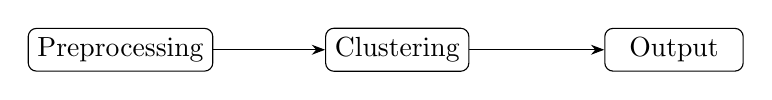
\begin{tikzpicture}
    \begin{scope}[every node/.style={draw, minimum size=2em, rectangle,
        rounded corners=3, minimum height=1.5em,
        minimum width=5em
        }]
        \node (a)at (0, 0){Preprocessing};
        \node (b)at (10em, 0){Clustering};
        \node (c)at (20em, 0){Output};
        % draw a arrow
        \draw[-{Stealth}] (a) -- (b);
        % comment: use tikz lib here: 
        \draw[-{Stealth}] (b) -- (c);
    \end{scope}
\end{tikzpicture}

\begin{itemize}
    \item 对公司进行聚类
    \item 在同一个投标出现过的公司才有可能聚类
    \item 公司之间聚类需要考虑时间维度,考虑历史投标数据
\end{itemize}

\subsection{Preprocessing}
\begin{itemize}
    \item Cleaning \& Imputation
    \item feature encoding
    \item 数据归一化
    \item 数据降维
\end{itemize}

\subsection{Clustering}
\begin{itemize}
    \item gower distance / similarity measures + K-medoids / spectral clustering
    \item any 2 companies on a bid: using xgboost to determine if they will co-occur
    \item DBSCAN
    \item Agglomerative hierarchical clustering
    \item GNN / DNN embedding + K-means
    \item GNN clustering
    \item deep clustering
\end{itemize}

Key ideas:
\begin{itemize}
    \item 扩展特征,采用gower distance 以及similarity distance,使用K-prototypes 聚类方式
    \item 考虑使用GNN进行聚类: 直接聚类或者使用K-prototypes 对GNN embedding 聚类
\end{itemize}

\subsection{Output}
\begin{itemize}
    \item 聚类结果
    \item 聚类结果可视化
\end{itemize}

\section{Phase 0.1}

\subsection{Distance}
\paragraph{Gower's distance}~\\

Gower's distance is used in statistics.

measure mixed types:
\begin{itemize}
    \item continuous
    \item binary
    \item ordinal
\end{itemize}

Value range: 0->1.

0 is the most similar. 

Definition:

Assuming p is number of features(descriptors).

\begin{equation}
    s_{ij} = \frac{\sum_{k=1}^p w_k s_k}{\sum_{k=1}^p w_k} = <W, S>
\end{equation}

For example, if feature k is ordinal:
\begin{equation}
    s_k = \frac{i - j}{max(s_k)- min(s_k)}
\end{equation}

question:

how to determine w?

Best practice is to use domain knowledge.

\paragraph{Historical Bis}~\\
How to encode historical bid data?
\begin{itemize}
    \item multihot encoding with freq as values
    \item GNN?
\end{itemize}

\subsection{Clustering}
\paragraph{public pretrained models}~\\

Is there any public models for this task?

% \begin{table}
% \caption{Table captions should be placed above the
% tables.}\label{tab1}
% \begin{tabular}{|l|l|l|}
% \hline
% Heading level &  Example & Font size and style\\
% \hline
% Title (centered) &  {\Large\bfseries Lecture Notes} & 14 point, bold\\
% 1st-level heading &  {\large\bfseries 1 Introduction} & 12 point, bold\\
% 2nd-level heading & {\bfseries 2.1 Printing Area} & 10 point, bold\\
% 3rd-level heading & {\bfseries Run-in Heading in Bold.} Text follows & 10 point, bold\\
% 4th-level heading & {\itshape Lowest Level Heading.} Text follows & 10 point, italic\\
% \hline
% \end{tabular}
% \end{table}


% ---- Bibliography ----
%
% BibTeX users should specify bibliography style 'splncs04'.
% References will then be sorted and formatted in the correct style.
%
\bibliographystyle{refs-style}
\bibliography{refs}
%
\end{document}